% This Latex poster uses the baposter class, originally from
% http://www.brian-amberg.de/uni/poster. Versions are found in several places.
% The files on which this version is based are from circulation within WASP
% and exact origins are not known.
%
% CONTENT
% To update the poster, modify the contents in the parts/ folder.
% The file header.tex contains convenience commands such as \title, \companylogo etc.
% Other files contain pure formatting.
%
% COLORS
% The following standard colors are defined: wasp_text, wasppink, waspgrey, waspblue
%
% Enjoy!
% Per Skarin, 2021

\documentclass[a1paper,portrait]{baposter}
\usepackage{lipsum}  
\usepackage{relsize}	% For \smaller
\usepackage{url}	% For \url
\usepackage{epstopdf}	% Included EPS files automatically converted to PDF to include with pdflatex
\usepackage[utf8]{inputenc} 
\usepackage{multirow}
\usepackage{booktabs}
\usepackage[labelfont=bf]{caption}
\usepackage{enumitem}
\usepackage{tcolorbox}
\usepackage{mathtools}

\usepackage{tgheros}
\usepackage{lmodern}
\usepackage[czech, linesnumbered, longend, noline]{algorithm2e}
\renewcommand{\figurename}{Obrázek}
\renewcommand{\tablename}{Tabulka}

% PATHS
\graphicspath{{template-images/}{content-images/}}

% FONTS AND COLORS
\renewcommand{\familydefault}{\rmdefault}
\newcommand{\mytitlefont}{\sffamily\bfseries\selectfont}
\newcommand{\mytextfont}{\rmfamily\normalfont\selectfont}
% Comment the four lines below to skip WASP fonts
% \usepackage{MinionPro}
% \usepackage{MyriadPro}
% \renewcommand{\mytitlefont}{\fontfamily{MyriadPro-LF}\selectfont }
% \renewcommand{\mytextfont}{\fontfamily{MinionPro-LF}\selectfont }

\definecolor{wasppink}{RGB}{203,166,169} 
\definecolor{waspgrey}{RGB}{88,89,91}
\definecolor{waspblue}{RGB}{26,141,173}
\definecolor{darkgreen}{rgb}{0,0.6,0}

\definecolor{spacecadet}{RGB}{37,52,79}
\definecolor{slategray}{RGB}{97,120,145}
\definecolor{tan}{RGB}{213,184,147}
\definecolor{coffe}{RGB}{111,77,56}
\definecolor{caputmortuum}{RGB}{99,32,36}

\definecolor{cookiesandcream}{RGB}{224,220,170}
\definecolor{teagrean}{RGB}{204,227,194}
\definecolor{laurelgreen}{RGB}{157,180,150}
\definecolor{milkchocholate}{RGB}{139,86,51}
\definecolor{metalicbronze}{RGB}{163,123,71}

\definecolor{wasp_text}{RGB}{66,80,82}
\colorlet{wasp_banner_light}{waspblue}
\colorlet{wasp_banner_dark}{waspgrey}

% LIST SETTINGS
\setlist{itemsep=.1em, leftmargin=1em}

% COMMANDS
\newcommand\thetitle{}\renewcommand\title[1]{\renewcommand\thetitle{#1}}
\newcommand\theauthor{}\renewcommand\author[1]{\renewcommand\theauthor{#1}}
\newcommand\thedepinfo{}\newcommand\depinfo[1]{\renewcommand\thedepinfo{#1}}
\newcommand\thesupervisors{}\newcommand\supervisors[1]{\renewcommand\thesupervisors{#1}}
\newcommand\theuniversitylogo{}\newcommand\universitylogo[1]{\renewcommand\theuniversitylogo{#1}}
\newcommand\thecompanylogo{}\newcommand\companylogo[1]{\renewcommand\thecompanylogo{#1}}


%%%%%%%%%%%%%%%%%%%%%%%%%%%%%%%%%%%%%%%%%%%%%%%%%%%%%%%%%%%%%%%%%%%%%%%%%%%%%%%
%%% Document Start %%%%%%%%%%%%%%%%%%%%%%%%%%%%%%%%%%%%%%%%%%%%%%%%%%%%%%%%%%%%
%%%%%%%%%%%%%%%%%%%%%%%%%%%%%%%%%%%%%%%%%%%%%%%%%%%%%%%%%%%%%%%%%%%%%%%%%%%%%%%

% Text to the left
\title{Kvantově inspirované optimalizační algoritmy}
\author{Bc. Tomáš Bártů}
\depinfo{Dept. of Automatic Control, A Project Within This Department}
\supervisors{doc. Ing. Michal Bidlo, Ph.D.}

% Logos on the right. Put the images in template-images/
\universitylogo{
\includegraphics[width=0.7\textwidth]{VUT-FIT-logo.pdf}}
\companylogo{\includegraphics[width=0.6\textwidth]{company/ericsson}}



\begin{document}

%%% General Poster Settings %%%%%%%%%%%%%%%%%%%%%%%%%%%%%%%%%%%%%%%%%%%%%%%%%%%
%%%%%% Eye Catcher, Title, Authors and University Images %%%%%%%%%%%%%%%%%%%%%%
\begin{poster}{
 % Show grid to help with alignment
 grid=false,
 % eyecatcher=false,
 % Column spacing
 colspacing=1em,
 columns=2,
 boxpadding=.5cm,
 % Color style
 headerColorOne=spacecadet,
 borderColor=spacecadet,
 headerFontColor=cyan!10!white,
 boxColorOne=teagrean,
 % Format of textbix
 textborder=rounded,
 % Format of text header
 headerborder=open,
 headershape=rounded,
 headershade=plain,
 background=plain,
 bgColorOne=cookiesandcream,
 headerheight=0.09\textheight}
%%% Eye Cacther %%%%%%%%%%%%%%%%%%%%%%%%%%%%%%%%%%%%%%%%%%%%%%%%%%%%%%%%%%%%%%%
{
	Eye Catcher, empty if option eyecatcher=false - unused
}
%%%% Title %%%%%%%%%%%%%%%%%%%%%%%%%%%%%%%%%%%%%%%%%%%%%%%%%%%%%%%%%%%%%%%%%%%%%
{
	\textcolor{spacecadet}{\mytitlefont \Huge \thetitle}
}
%%% Authors %%%%%%%%%%%%%%%%%%%%%%%%%%%%%%%%%%%%%%%%%%%%%%%%%%%%%%%%%%%%%%%%%%%
{
  \vspace{0.5em}
  \textcolor{spacecadet}{\Large \theauthor\\
	% \large \thedepinfo\\
	Vedoucí: \thesupervisors\\
	}
}
%%% Logo %%%%%%%%%%%%%%%%%%%%%%%%%%%%%%%%%%%%%%%%%%%%%%%%%%%%%%%%%%%%%%%%%%%%%%
{
  \begin{minipage}{8cm}
   \centering
   \vspace{0.5cm}
	    % \theuniversitylogo\vspace{0.25cm}\par
		  % \thecompanylogo
  \end{minipage}
}

%%%%%%%%%%%%%%%%%%%%%%%%%%%%%%%%%%%%%%%%%%%%%%%%%%%%%%%%%%%%%%%%%%%%%%%%%%%%%%
%%% Now define the boxes that make up the poster
%%%---------------------------------------------------------------------------
%%% Each box has a name and can be placed absolutely or relatively.
%%% The only inconvenience is that you can only specify a relative position 
%%% towards an already declared box. So if you have a box attached to the 
%%% bottom, one to the top and a third one which should be inbetween, you 
%%% have to specify the top and bottom boxes before you specify the middle 
%%% box.
%%%%%%%%%%%%%%%%%%%%%%%%%%%%%%%%%%%%%%%%%%%%%%%%%%%%%%%%%%%%%%%%%%%%%%%%%%%%%%

%%%%%%%%%%%%%%%%%%%%%%%%%%%%%%%%%%%%%%%%%%%%%%%%%%%%%%%%%%%%%%%%%%%%%%%%%%%%%%
  \headerbox{\mytitlefont Motivace a cíle}{name=description,column=0,row=0,span=2}{
  \mytextfont
%%%%%%%%%%%%%%%%%%%%%%%%%%%%%%%%%%%%%%%%%%%%%%%%%%%%%%%%%%%%%%%%%%%%%%%%%%%%%%
  % Put the motivation behind and goals of the research here
\large
Tato práce se zaměřuje na srovnání kvantově inspirovaných evolučních algoritmů (\emph{QIEA}) využívajících principů kvantové fyziky při řešení kombinatorického problému batohu ve variantě 0/1.
Cílem je ověřit schopnosti těchto algoritmů a vytvořit srovnávací studii jejich výkonnosti.
V průběhu práce byl rovněž navržen a otestován vlastní vylepšený algoritmus \emph{QIPSO}.

}

%%%%%%%%%%%%%%%%%%%%%%%%%%%%%%%%%%%%%%%%%%%%%%%%%%%%%%%%%%%%%%%%%%%%%%%%%%%%%%
  \headerbox{\mytitlefont Problém a přístup}{name=motivation,column=0,row=0,span=1, below=description}{
%%%%%%%%%%%%%%%%%%%%%%%%%%%%%%%%%%%%%%%%%%%%%%%%%%%%%%%%%%%%%%%%%%%%%%%%%%%%%%
  \mytextfont
  % The methods that you use goes here
{\large\underline{\textbf{Problém batohu 0/1}}} \\[0.5em]
Každá položka může být vybrána nejvýše jednou tak, aby celková hodnota vybrané podmnožiny položek byla maximální a součet jejich vah nepřesáhl kapacitu batohu.
\begin{equation}
  \max \sum_{i=1}^{n} v_i x_i
  \quad \text{s podmínkou} \quad \sum_{i=1}^{n} w_i x_i \leq C,
  \quad x_i \in \{0,1\}
\end{equation}

{\large\underline{\textbf{Kvantová reprezentace řešení}}} \\[0.5em]
V binárním \emph{QIEA} je qubit (jedinec) popsán dvojicí koeficientů $\alpha$ a $\beta$, přičemž systém složený z $m$ qubitů (populace) lze vyjádřit jako:
\label{eq:quantum-representation} 
\begin{equation}
  \begin{bmatrix}
    \alpha_1 & \alpha_2 & \dots & \alpha_m \\ \beta_1 & \beta_2 & \dots & \beta_m
  \end{bmatrix},
  \quad \text{kde} \quad \forall i \in \left\{ 1,2,\dots,m \right\}: \quad \alpha_i^2 + \beta_i^2 = 1.
\end{equation}
Pravděpodobnostní koeficienty $\alpha_i$ a $\beta_i$ $i$-tého qubitu jsou aktualizovány pomocí kvantového rotačního hradla, viz obrázek~\ref{fig:rotation-gate}:
\begin{equation}
  \label{eq:rotation-gate-angles}
  \begin{bmatrix} 
    \alpha_i' \\ 
    \beta_i'
  \end{bmatrix} = 
  \begin{bmatrix} 
    \cos{\left( \Delta\theta_i \right)} & - \sin{\left( \Delta\theta_i \right)} \\
    \sin{\left( \Delta\theta_i \right)} & \cos{\left( \Delta\theta_i \right)}
  \end{bmatrix} 
  \begin{bmatrix} 
    \alpha_i \\ 
    \beta_i 
  \end{bmatrix},
\end{equation}
kde je úhel $\Delta\theta_i$ určen ná základě tabulky~\ref{tab:look-up-table-Delta}, a to podle aktuálně pozorovaného řešení $x_i$ a nejlepšího známého řešení $b_i$:

\begin{minipage}{0.49\linewidth}
    \centering
    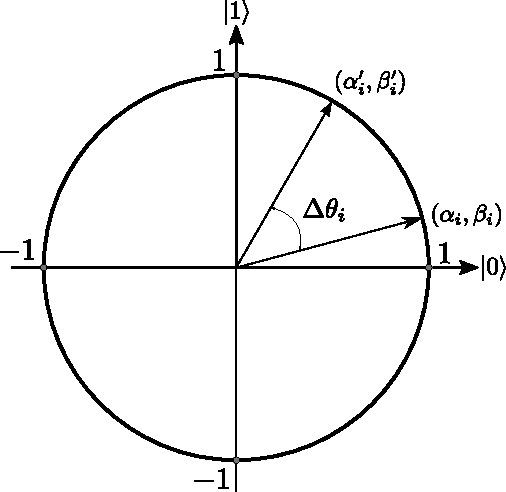
\includegraphics[width=0.9\linewidth]{rotation-gate.pdf}
    \captionof{figure}{Rotační hradlo.}
    \label{fig:rotation-gate}
\end{minipage}
\hfill
\begin{minipage}{0.49\linewidth}
    \centering
    \begin{tabular}{c c|c}
    \toprule
    $x_i$ & $b_i$ & $\Delta\theta_i$ \\
    \midrule
    1 & 1 & 0 \\
    0 & 1 & $a$ \\
    0 & 0 & 0 \\
    1 & 0 & $-a$ \\
    \bottomrule
    \end{tabular}
    \captionof{table}{Tabulka pro odvození $\Delta\theta_i$.}
    \label{tab:look-up-table-Delta}
\end{minipage}

\vspace{0.5em}

{\large\underline{\textbf{Použité algoritmy}}} \\[0.5em]
V rámci experimentální části byly testovány čtyři \emph{QIEA}:
\begin{itemize}
  \item \emph{QIGA} (kvantově inspirovaný genetický algoritmus),
  \item \emph{QISA} (kvantově inspirované simulované žíhání),
  \item \emph{QSE} (kvantově inspirovaný částicový roj)
  \item a vlastní navržená varianta \emph{QIPSO} vycházející z \emph{QSE}.
\end{itemize}
Cílem bylo porovnat jejich schopnost řešit problém batohu 0/1 při různých velikostech instancí.
Pro shrnutí parametrů testovaní vizte tabulka~\ref{tab:experiment-settings}.

\vspace{0.5em}

\begin{minipage}{\linewidth}
  \centering
  \begin{tabular}{|l|l|}
  \hline
  \textbf{Položka} & \textbf{Hodnota} \\
  \hline
  Testované algoritmy & QIGA, QISA, QSE, QIPSO \\
  \hline
  Instance & 100, 250, 500, 1000, 2000, 5000 položek \\
  \hline
  Počet běhů & 30 na každé nastavení \\
  \hline
  Fitness evaluací & 10 000 na běh \\
  \hline
  \end{tabular}
  \captionof{table}{Parametry experimentálního nastavení.}
  \label{tab:experiment-settings}
\end{minipage}
\vspace{0.5em}

}

%%%%%%%%%%%%%%%%%%%%%%%%%%%%%%%%%%%%%%%%%%%%%%%%%%%%%%%%%%%%%%%%%%%%%%%%%%%%%%
  \headerbox{\mytitlefont Algoritmus 1: QIPSO}{name=qipso,column=1,row=0,span=1, below=description}{
%%%%%%%%%%%%%%%%%%%%%%%%%%%%%%%%%%%%%%%%%%%%%%%%%%%%%%%%%%%%%%%%%%%%%%%%%%%%%%
    \mytextfont
    \begin{tcolorbox}[colframe=coffe, width=\textwidth, left=-0.2em, right=-1.65em, top=1mm, bottom=1mm]
    % \IncMargin{-1.7em}
    \begin{algorithm}[H]
      \footnotesize	
      $t \gets 0$\;
      Inicializace kvantové populace $Q(t)$ s amplitudami $\frac{1}{\sqrt{2}}$\;
      Inicializace rychlosti $V(t) \gets 0$\;
      Nastavení globálního nejlepší řešení $B(t)$\;
      \While{$t < t_{\max}$}{
          $t \gets t + 1$\;
          \For{$j = 1$ \textbf{to} $n$}{
              Pozorování kvantového chromozomu $p_j(t)$ z $Q(t-1)$\;
              Oprava $p_j(t)$ tak, aby splňovalo kapacitní omezení\;
              Ohodnocení řešení $f_j(t)$\;
          }
          Aktualizace osobního nejlepší řešení částic\;
          Aktualizace globálního nejlepší řešení $B(t)$\;
          \For{$j = 1$ \textbf{to} $n$}{
              Generování náhodných koeficientů $r_1, r_2 \in \langle 0, 1\rangle$\;
              Aktualizace rychlosti:
              $V_j(t) \gets \text{friction} \times V_j(t-1) + c_1 r_1 (p_{\text{best},j} - p_j(t)) + c_2 r_2 (g_{\text{best}} - p_j(t))$\;
              Aplikace kvantového rotačního hradla na $Q_j(t)$ s úhlem $V_j(t)$;
          }
      }
      \Return nejlepší nalezené řešení $B(t)$\;
    \end{algorithm}
\end{tcolorbox}
}

%%%%%%%%%%%%%%%%%%%%%%%%%%%%%%%%%%%%%%%%%%%%%%%%%%%%%%%%%%%%%%%%%%%%%%%%%%%%%%
  \headerbox{\mytitlefont Vybrané výsledky}{name=goal,column=1,row=0,span=1, below=qipso}{
%%%%%%%%%%%%%%%%%%%%%%%%%%%%%%%%%%%%%%%%%%%%%%%%%%%%%%%%%%%%%%%%%%%%%%%%%%%%%%
  \mytextfont
  \renewcommand{\figurename}{Graf}

\vspace{-0.5em}

\begin{minipage}{\linewidth}
    \centering
    \begin{tikzpicture}
        \node[ draw=coffe, line width=2pt, inner sep=0pt ] 
        {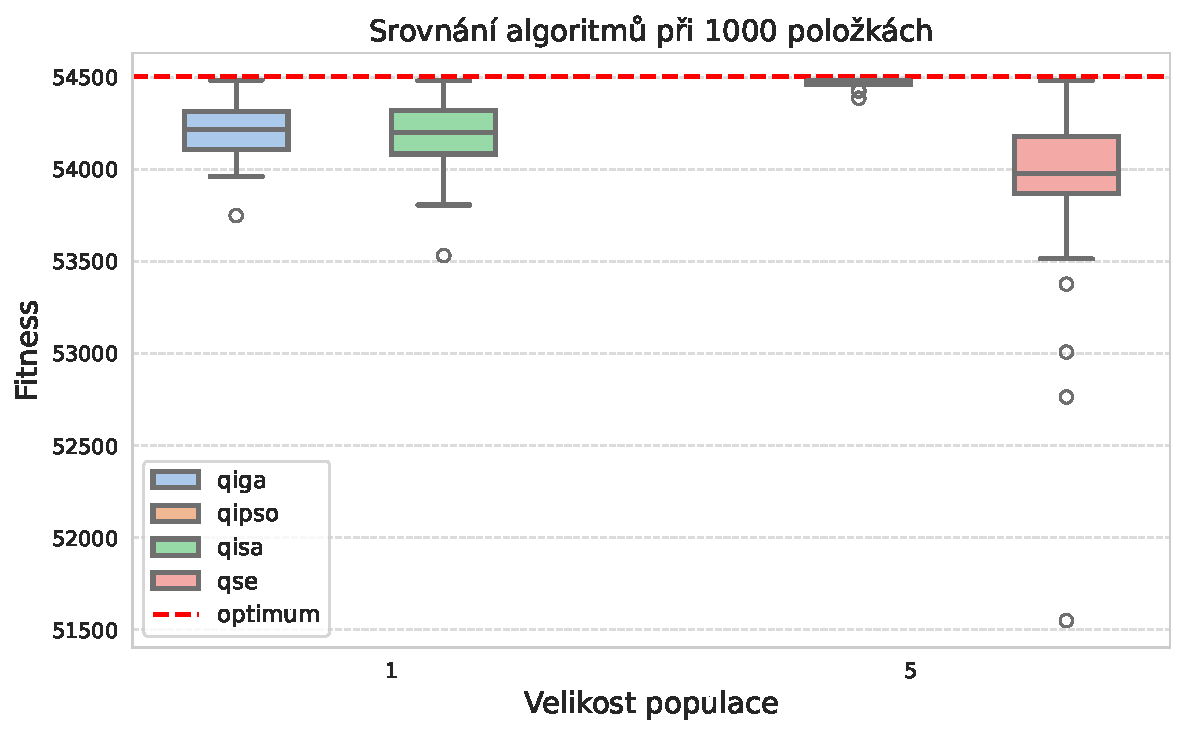
\includegraphics[width=0.9\linewidth]{best_all_qiea_1000.pdf}};
    \end{tikzpicture}
	{\vspace{-0.5em}}
    \captionof{figure}{Výsledky experimentu na instanci s 1000 položkami.}
    \label{fig:qiea-2000}
\end{minipage}

\vspace{0.6em}

\begin{minipage}{\linewidth}
    \centering
    \begin{tikzpicture}
        \node[ draw=coffe, line width=2pt, inner sep=0pt ] 
        {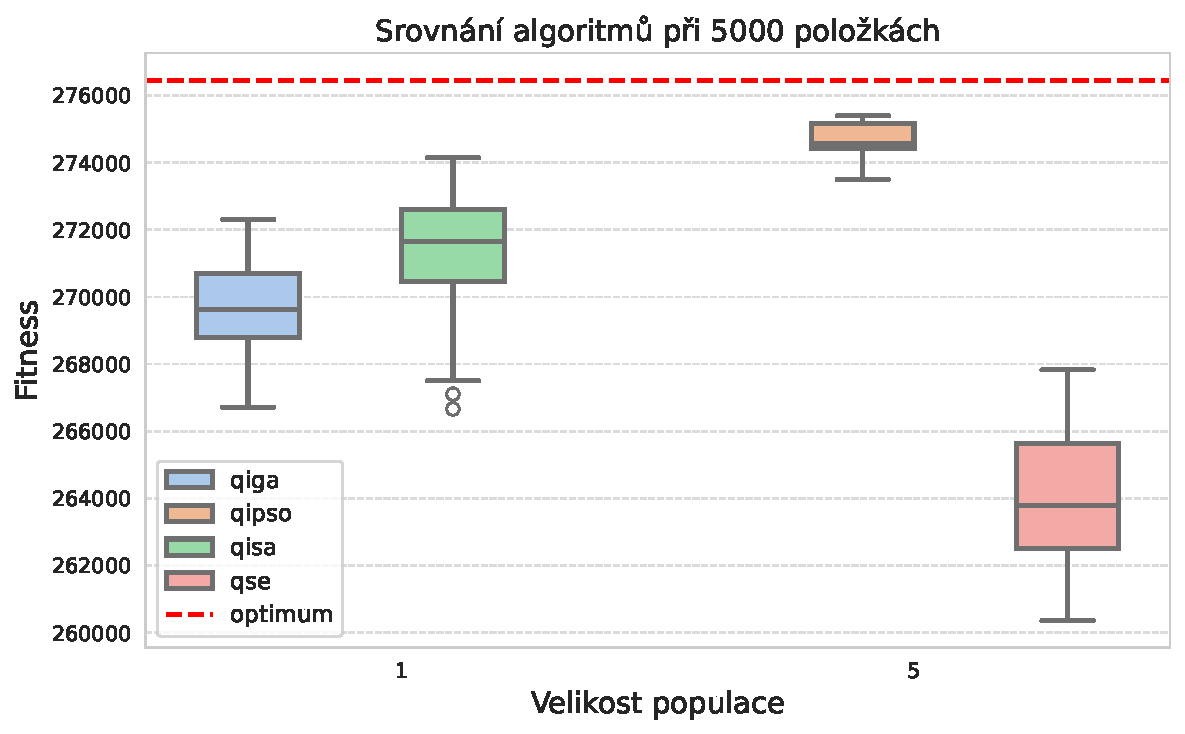
\includegraphics[width=0.9\linewidth]{best_all_qiea_5000.pdf}};
    \end{tikzpicture}
	{\vspace{-0.5em}}
    \captionof{figure}{Výsledky experimentu na instanci s 5000 položkami.}
    \label{fig:qiea-5000}
\end{minipage}

\vspace{0.55em}

}

% %%%%%%%%%%%%%%%%%%%%%%%%%%%%%%%%%%%%%%%%%%%%%%%%%%%%%%%%%%%%%%%%%%%%%%%%%%%%%%
%   \headerbox{Literatura}{headerColorOne=caputmortuum, borderColor=caputmortuum, name=results,column=0,row=0,span=1, below=qipso }{
% %%%%%%%%%%%%%%%%%%%%%%%%%%%%%%%%%%%%%%%%%%%%%%%%%%%%%%%%%%%%%%%%%%%%%%%%%%%%%%
% 	\mytextfont
%   \small
\vspace{-0.5cm}
\fcolorbox{white}{white}{\hspace{-0.5cm}\parbox{0.1\linewidth}{\centering [1]}\parbox{1.3cm}{}\parbox{0.7\linewidth}{\footnotesize\smaller Five Challenges in Cloud-Enabled Intelligence and Control\\\tiny T. Abdelzaher, Y. Hao, K. Jayarajah, A. Misra, S. Yao, P. Skarin, D. Weerakoon and K. {\AA}rz{\'e}n\\ACM Transactions on Internet Technology, 2019}}\par\vspace{-0.4cm}
	
\fcolorbox{white}{white}{\hspace{-0.5cm}\parbox{0.1\linewidth}{\centering [2]}\parbox{1.3cm}{}\parbox{0.7\linewidth}{\footnotesize\smaller Towards Mission-Critical Control at the Edge and Over 5G\\\tiny Per Skarin, William Tärneberg, Karl-Erik Årzén, Maria Kihl\\Best paper award, IEEE Services (EDGE), 2-7 July, 2018, San Fran., CA, USA}}\par\vspace{-0.25cm}
	
\fcolorbox{white}{white}{\hspace{-0.5cm}\parbox{0.1\linewidth}{\centering [5]}\parbox{1.3cm}{}\parbox{0.7\linewidth}{\footnotesize\smaller Cloud-based model predictive control with variable horizon\\\tiny Per Skarin, Johan Eker, Karl-Erik Årzén\\Subm. to 21st World Congress of the International Federation of Automatic Control, 2020}}\par\vspace{-0.3cm}

% }

\headerbox{}{name=foottext, column=0, span=2, above=bottom,headerColorOne=caputmortuum, textborder=none,headerborder=none,boxheaderheight=0pt,boxColorOne=caputmortuum}{
\includegraphics[height=1cm]{VUT-FIT-logo.pdf} \hfill 
\includegraphics[height=1cm]{ExcelAtFIT-logo.pdf}}


\end{poster}
\end{document}
